\documentclass[tikz,border=5pt]{standalone}
\usepackage{tikz}
\usetikzlibrary{positioning,calc}

\begin{document}
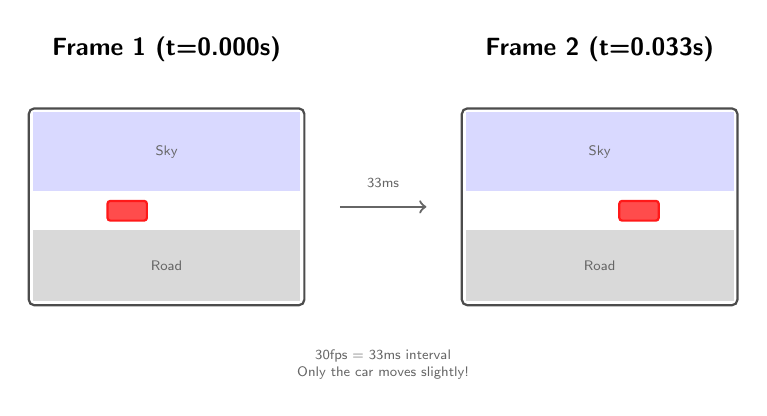
\begin{tikzpicture}[
    frame/.style={draw=black!70, thick, minimum width=3.5cm, minimum height=2.5cm, rounded corners=2pt},
    sky/.style={fill=blue!15},
    road/.style={fill=gray!30},
    label/.style={font=\small\sffamily\bfseries},
    sublabel/.style={font=\tiny\sffamily, text=black!60},
    car/.style={fill=red!70, draw=red!90, thick, rounded corners=1pt}
]

% Frame 1
\begin{scope}[shift={(0,0)}]
    \node[label] at (0, 2.0) {Frame 1 (t=0.000s)};

    % Frame box
    \draw[frame] (-1.75, -1.25) rectangle (1.75, 1.25);

    % Sky area
    \fill[sky] (-1.7, 0.2) rectangle (1.7, 1.2);
    \node[sublabel] at (0, 0.7) {Sky};

    % Road area
    \fill[road] (-1.7, -1.2) rectangle (1.7, -0.3);
    \node[sublabel] at (0, -0.75) {Road};

    % Car
    \node[car, minimum width=0.5cm, minimum height=0.25cm] at (-0.5, -0.05) {};
\end{scope}

% Arrow
\draw[->, thick, black!60] (2.2, 0) -- (3.3, 0);
\node[sublabel] at (2.75, 0.3) {33ms};

% Frame 2
\begin{scope}[shift={(5.5,0)}]
    \node[label] at (0, 2.0) {Frame 2 (t=0.033s)};

    % Frame box
    \draw[frame] (-1.75, -1.25) rectangle (1.75, 1.25);

    % Sky area
    \fill[sky] (-1.7, 0.2) rectangle (1.7, 1.2);
    \node[sublabel] at (0, 0.7) {Sky};

    % Road area
    \fill[road] (-1.7, -1.2) rectangle (1.7, -0.3);
    \node[sublabel] at (0, -0.75) {Road};

    % Car (moved right)
    \node[car, minimum width=0.5cm, minimum height=0.25cm] at (0.5, -0.05) {};
\end{scope}

% Explanation
\node[sublabel, text width=4cm, align=center] at (2.75, -2.0) {30fps = 33ms interval\\Only the car moves slightly!};

\end{tikzpicture}
\end{document}
